% !TEX root=../main.tex
\documentclass[beamer]{standalone}
\begin{document}
% ==============================================================
% Method : Gradient Descenet Explanations - 0 
% ==============================================================   
\begin{frame}{Method}
    \framesubtitle{Laplacian operator on the image kernel}
        \begin{figure}[t]
        \centering
            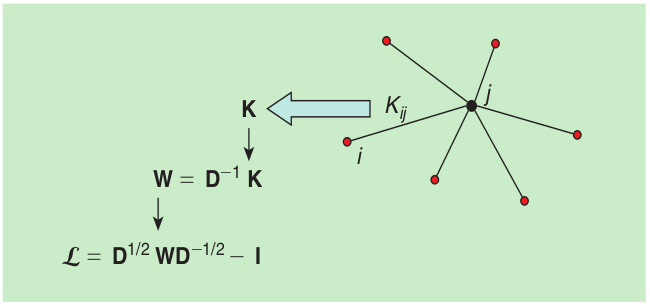
\includegraphics[width=6cm]{./figures/image-kernel-laplacian.png}
            \caption{from: \emph{"A Tour of Modern Image Filtering"}}
        \end{figure}
        \begin{itemize}
            \item Filtering problem, the convenient vector form $z(x)=Wy$
        \end{itemize}
        \begin{table}
            \centering
            \resizebox{12cm}{!}{
            \begin{tabular}{ | c | c | c | c | } \hline
                Graph Laplacian & Symmetric                & DC eigenvector & Spectral Range \\ \hline
                Un-normalized   & $D - K$                  & Yes            & [0, n] \\ \hline
                Normalized      & $I - D^{-1/2}KD^{-1/2}$  & No             & [0, 2] \\ \hline  
            \end{tabular}}
        \end{table}

    % note %
    \note[item] {
    }
\end{frame}

\begin{frame}{Method}
    \framesubtitle{The choice on step length}
        \begin{equation}
            x \leftarrow x - \eta \textcolor{red}{(I + \lambda L)^{-p}} {\diffp{\Phi}{x}}
        \end{equation}
        \begin{itemize}    
            \item Need for choosing step size $\lambda$
            \item Step size can be chosen with weak wolfe condiiton, goldstein condition and backtracking ..
            \begin{itemize}
                \item But, we need the function evaluation for each step length
                \item In the current case, our function is MSE between target and rendering image
            \end{itemize}
            \item Now just using the scaled step size from an original adam optimizer
            \begin{itemize}
                \item On the "Large steps in the inverse rendering of Geometry" $\lambda$ is set as from 15 to 50
                \item On the "Laplacian Smooth Gradient Descent", the authors shows a proof on optimal value
            \end{itemize}
        \end{itemize}
\end{frame}

\end{document}